\subsection{Время над порогом}\label{section:secToT}

Время над порогом (ToT --- time over threshold) --- это параметр найденного хита, содержащий в себе, при нормальной работе, информацию об амплитуде зарегистрированного сигнала. В системе считывания и сбора данных CBM~RICH ToT может быть использовано для улучшения временного разрешения путём коррекции времени пересечения порога с учетом амплитуды (walk correction), а также для повышения качества отделения однофотоэлектронного сигнала от шума. На рисунке~\ref{fig:ToTdata} показано типичное распределение ToT, измереное с помощью лазера в лабораторных условиях. Вопреки ожиданиям, это распределение имеет несколько пиков. Такая структура, согласно~\cite{ToTinNoise}, может быть объяснена наличием периодической наводки как на входе дискриминатора, так и между выходом дискриминатора и входом ВЦП. На рисунке~\ref{fig:ToTscope} показан экран цифрового осциллографа в режиме накопления сигналов, полученных путем подключения активного зонда к выходу PADIWA. Видно, что сгущение сигналов соответствует наблюдаемым пикам в распределении ToT; имеет место проблема недостаточности амплитуды одноэлектронного сигнала для устойчивой генерации логической единицы; имеется периодическая наводка на выходе дискриминатора, но ее недостаточно для объяснения наблюдаемой картины; преобладание определенных длительностей логических сигналов позволяет предположить наличие периодической структуры во входном сигнале. Все это говорит о необходимости подстройки аналоговой части для формирования на входе PADIWA более чистого сигнала большей амплитуды и о защите соединения между дискриминатором и ВЦП от наводок. Подобные изменения будут, с учетом результатов данной работы, реализованы в следующем прототипе платы передней электроники, называемом DIRICH~\cite{}.
%Из такой формулировки кажется, что это прототип называется DIRICH. А на самом деле это итоговая плата передней электроники так называется.

\begin{figure}
\begin{minipage}[b]{0.495\textwidth}
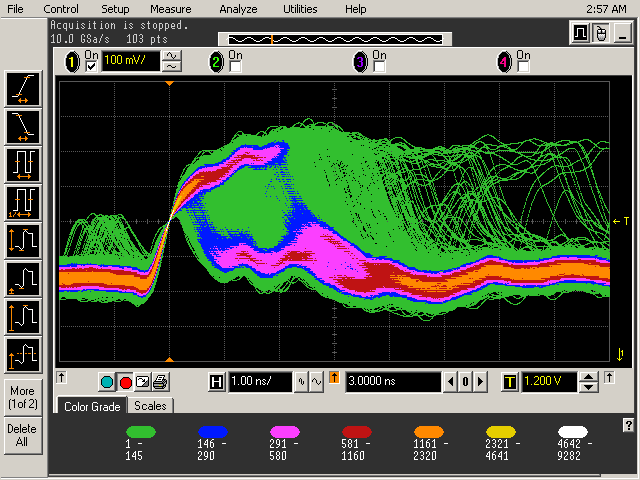
\includegraphics[width=1.0\textwidth]{pictures/Scope_additional.png}
\end{minipage}
\hspace{0.01\textwidth}
\begin{minipage}[b]{0.495\textwidth}
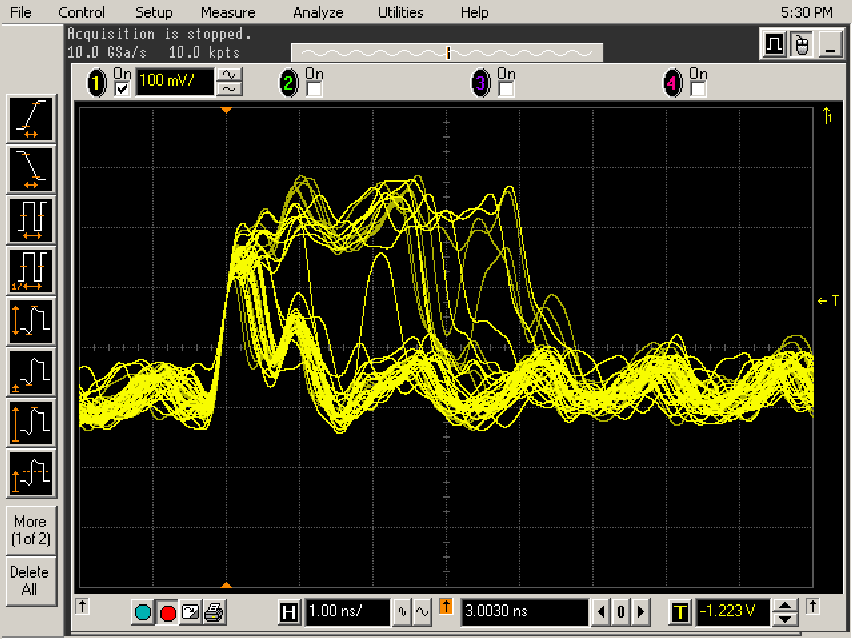
\includegraphics[width=1.0\textwidth]{pictures/Scope2.png}
\end{minipage}
\caption{}
\label{fig:ToTscope}
\end{figure}

\begin{figure}
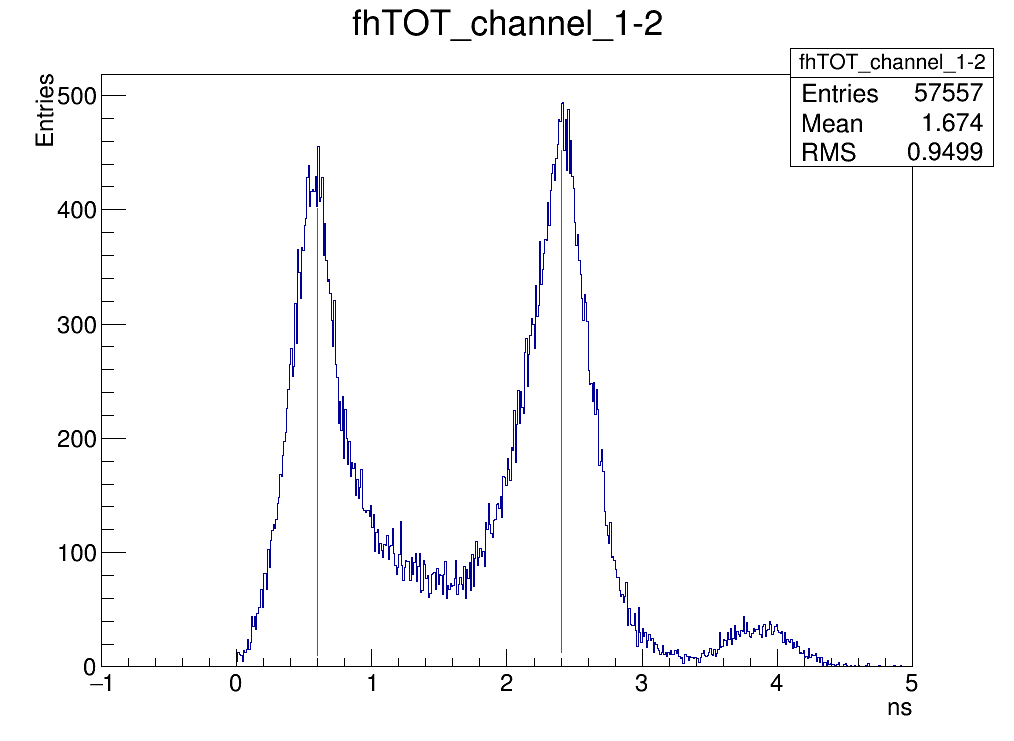
\includegraphics[width=0.6\textwidth]{pictures/Scope_vs_data-data.png}
\caption{Типичное распределение ToT.}
\label{fig:ToTdata}
\end{figure}

%Зачем запятая?
%"разделение сигналов и шумов" либо "отделение сигнала от шума", не так?
Отметим, что указанные проблемы не являются критичными в случае CBM~RICH, и продемонстрированные в данной работе параметры достаточны для уверенного поиска колец. Тем не менее, улучшение разделения сигнала от шума и повышение эффективности регистрации поможет создать необходимый запас надежности для долговременной работы детектора в условиях постепенной деградации оптических свойств радиатора, зеркал и фотодетекторов.
